% =====================================================================
%  Short talk (7 slides) cut from head-sets-simple-slides.tex, i.e. from
%  paper/head-sets-simple-design.tex: background, the two published methods,
%  main idea (decoding + attention, combination chosen on held-out items),
%  main comparison, the tests beyond the identification prompts at 40 heads.
%  Left out on purpose: the step-by-step ladder, feature contributions,
%  layers, controls, task types, overlap between prompting styles.
%  Numbers are copied from paper/tables/design_{ladder,own,wordings_transfer,
%  wordings_reid,examples,summed,unseen}.tex.
%  Compile with Tectonic from this folder:  tectonic head-sets-simple-short.tex
% =====================================================================
\documentclass[aspectratio=169,11pt,xcolor=table]{beamer}

\usetheme{default}
\usefonttheme{professionalfonts}
\setbeamertemplate{navigation symbols}{}
\setbeamertemplate{footline}{\hfill\scriptsize\color{gray}\insertframenumber\hspace{1.2em}\vspace{0.6em}}
\setbeamertemplate{itemize items}{\textbullet}

\usepackage{booktabs,array,amsmath,amssymb}
\usepackage{tikz}
\usetikzlibrary{positioning,arrows.meta,calc}
\usepackage{pgfplots}
\pgfplotsset{compat=1.18}

% ---- colours (same as the long deck) ----------------------------------
\definecolor{ink}{HTML}{222222}
\definecolor{accent}{HTML}{1F6FB2}
\definecolor{soft}{HTML}{F2F4F7}
\definecolor{cYangL}{HTML}{2A78D6}
\definecolor{cYangJ}{HTML}{EDA100}
\definecolor{cD}{HTML}{E87BA4}
\definecolor{cSel}{HTML}{1BAF7A}
\definecolor{cCaus}{HTML}{EB6834}
\definecolor{cCausG}{HTML}{008300}
\definecolor{cBOS}{HTML}{B8B8B8}
\definecolor{cTask}{HTML}{F4B942}
\definecolor{cOther}{HTML}{F6D7B0}
\definecolor{cQuery}{HTML}{9CC3E6}
\definecolor{cMark}{HTML}{C79BD8}
\definecolor{cStop}{HTML}{CFE8C4}
\definecolor{cPunct}{HTML}{A8DCD1}
\definecolor{cLast}{HTML}{F08A80}
\definecolor{acc}{HTML}{1BAF7A}

\setbeamercolor{frametitle}{fg=ink}
\setbeamercolor{normal text}{fg=ink}
\setbeamercolor{structure}{fg=accent}
\setbeamerfont{frametitle}{series=\bfseries,size=\Large}

\newcommand{\takeaway}[1]{\vfill
  \begin{beamercolorbox}[wd=\textwidth,sep=6pt]{takeaway}\small #1\end{beamercolorbox}}
\setbeamercolor{takeaway}{bg=soft,fg=ink}

\newcommand{\cv}[1]{\pgfmathtruncatemacro{\cvshade}{#1*70}\edef\cvcmd{\noexpand\cellcolor{acc!\cvshade!white}}\cvcmd#1}
\newcommand{\Sel}{\textcolor{cSel}{\textbf{Combined}}}
\newcommand{\Causal}{\textcolor{cCaus}{Causal}}
\newcommand{\CausalG}{\textcolor{cCausG}{Causal $-$ generic}}
\newcommand{\nl}{\textbackslash n}
\newcommand{\tok}[2]{\tikz[baseline=(t.base)]\node[fill=#1,rounded corners=2pt,inner sep=1.8pt,font=\ttfamily\footnotesize](t){\strut #2};}

\title{Small Attention-Head Sets That Trigger Simple Tasks}
\subtitle{Identifying heads by what they decode, where they attend and what they cause\\
\small Llama-3.1-8B-Instruct, 14 tasks}
\author{Filippo Merlo}
\date{November 2026}

\begin{document}

% =====================================================================
\begin{frame}
\titlepage
\end{frame}

% =====================================================================
\begin{frame}{Background: a task triggered by a few heads}
\begin{columns}[c]
\column{0.46\textwidth}
\begin{itemize}
\item Prior work: part of a \textbf{task representation} sits in the outputs of a
      \textbf{few attention heads}.
\item[]
\item \textbf{Goal:} identify those heads
  \begin{itemize}\small
  \item from unpatched forward passes,
  \item as well as by their causal effect,
  \item one set per task or for all tasks.
  \end{itemize}
\item[]
\item \textbf{14 simple tasks} (Yang et al., 2026). Sets of 10--120 heads, identified and tested on
      separate halves of the items.
\end{itemize}

\column{0.5\textwidth}
\centering
\textbf{How we test a set}\\[6pt]
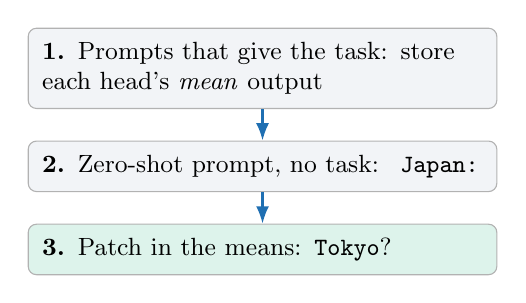
\begin{tikzpicture}[
  box/.style={draw=gray!60,rounded corners=3pt,fill=soft,align=left,font=\small,inner sep=5pt,text width=5.6cm},
  arr/.style={-{Latex[length=2.2mm]},thick,accent}]
\node[box](a){\textbf{1.} Prompts that give the task: store each head's \emph{mean} output};
\node[box,below=0.4cm of a](b){\textbf{2.} Zero-shot prompt, no task: \texttt{\ Japan:}};
\node[box,below=0.4cm of b,fill=cSel!15](c){\textbf{3.} Patch in the means: \texttt{Tokyo}?};
\draw[arr](a)--(b); \draw[arr](b)--(c);
\end{tikzpicture}
\end{columns}
\takeaway{A set \emph{triggers} the task if its means make the zero-shot prompt answer it,
and a related task's means do not.}
\end{frame}

% =====================================================================
\begin{frame}{Background: two published ways to identify heads}
\begin{columns}[T]
\column{0.47\textwidth}
\textbf{Lexical task heads}\\{\small Yang et al., 2026}
\begin{itemize}
\item Keep heads whose logit-lens top tokens match \textbf{predefined} task terms.
\item Cheap, but triggers few items (0.14), almost only fact tasks.
\end{itemize}

\column{0.47\textwidth}
\textbf{Causal score}\\{\small Davidson et al., 2025}
\begin{itemize}
\item Patch \textbf{one head at a time} into a prompt whose instruction is replaced.
\item Stronger (their 20-head vector: 0.29), but costly:
      about \textbf{61{,}000} patched passes per task.
\item Some top heads are \textbf{generic} (same push on every task); we also drop them.
\end{itemize}
\end{columns}

\takeaway{Reading heads is cheap but misses tasks; patching works but is costly.}
\end{frame}

% =====================================================================
\begin{frame}{Main idea: what a head decodes + where the last token attends}
\textbf{D}: decodes words of the task's list. Heads read with \textbf{J-head} (Head-JLens), through the
layers that follow; the list \emph{taken from what heads decode} (TF-IDF against WikiText).\\
{\footnotesize\color{gray}country--capital: city, cities, country, answer, countries, town, \dots, capital}

\vspace{0.7em}
\textbf{Attention} from the last token to each segment:\\[5pt]
\centering
\tok{cBOS}{<bos>}\,\tok{cOther}{Task}\tok{cPunct}{:}\,\tok{cOther}{given}\,\tok{cStop}{the}\,\tok{cTask}{country}\tok{cPunct}{,}\,\tok{cTask}{answer}\,\tok{cStop}{the}\,\tok{cTask}{capital}\,\tok{cStop}{of}\,\tok{cStop}{the}\,\tok{cTask}{country}\tok{cPunct}{.}\,\tok{cMark}{Q:}\,\tok{cQuery}{France}\,\tok{cMark}{\nl A}\tok{cLast}{:}

\vspace{0.5em}
\footnotesize
\begin{tabular}{@{}l@{\hspace{0.4em}}l@{\hspace{1.6em}}l@{\hspace{0.4em}}l@{\hspace{1.6em}}l@{\hspace{0.4em}}l@{\hspace{1.6em}}l@{\hspace{0.4em}}l@{}}
\textbf{B} & all but \tok{cBOS}{<bos>} & \tok{cTask}{T} & task words & \tok{cOther}{O} & other words & \tok{cStop}{S} & stopwords \\[3pt]
\tok{cPunct}{P} & punctuation & \tok{cMark}{M} & markers & \tok{cQuery}{Q} & query & \tok{cLast}{L} & last token \\
\end{tabular}

\vspace{0.6em}
\raggedright\small
\textbf{Combine:} average each head's rank over the features, keep the top $N$.
The combination (of 511) is chosen on the \emph{other} half of the items: \Sel.\\
\footnotesize At 40 heads: DBTSPL per task, DBTM shared.
\takeaway{Once the combination is fixed, no patching: at most 300 forward passes per task.}
\end{frame}

% =====================================================================
\begin{frame}{Main result: accuracy on the zero-shot prompt}
\centering
\pgfplotsset{
  every axis/.style={width=7.0cm,height=4.45cm,
    xmin=4,xmax=126,ymin=0,ymax=0.8,xtick={10,20,40,60,80,100,120},
    ytick={0,0.2,0.4,0.6,0.8},grid=major,grid style={gray!20},
    tick label style={font=\scriptsize},label style={font=\footnotesize},
    title style={font=\small\bfseries},xlabel={heads in the set ($N$)}},
  sYL/.style={cYangL,thick,mark=*,mark size=1.4pt},
  sYJ/.style={cYangJ,thick,mark=square*,mark size=1.3pt},
  sD/.style={cD,thick,mark=triangle*,mark size=1.7pt},
  sSel/.style={cSel,ultra thick,mark=diamond*,mark size=2.0pt},
  sC/.style={cCaus,thick,mark=triangle*,mark size=1.7pt,mark options={rotate=180}},
  sCG/.style={cCausG,thick,mark=pentagon*,mark size=1.6pt}}
\pgfplotslegendfromname{lg}\\[2pt]
\begin{tikzpicture}
\begin{axis}[title={One set per task},ylabel={accuracy}]
\addplot[sYL]  coordinates {(10,0.11)};
\addplot[sYJ]  coordinates {(10,0.14)(20,0.17)};
\addplot[sD]   coordinates {(10,0.20)(20,0.24)(40,0.33)(60,0.37)(80,0.37)(100,0.32)(120,0.26)};
\addplot[sSel] coordinates {(10,0.24)(20,0.42)(40,0.64)(60,0.67)(80,0.66)(100,0.66)(120,0.67)};
\addplot[sC]   coordinates {(10,0.25)(20,0.33)(40,0.41)(60,0.46)(80,0.53)(100,0.56)(120,0.61)};
\addplot[sCG]  coordinates {(10,0.31)(20,0.40)(40,0.48)(60,0.52)(80,0.53)(100,0.55)(120,0.58)};
\end{axis}
\end{tikzpicture}\hspace{0.3cm}%
\begin{tikzpicture}
\begin{axis}[title={One set for all 14 tasks},yticklabels={},
  legend to name=lg,legend columns=3,
  legend cell align=left,
  legend style={font=\scriptsize,draw=none,/tikz/every even column/.append style={column sep=10pt}}]
\addplot[sYL]  coordinates {(10,0.02)(20,0.04)(40,0.12)(60,0.12)(80,0.03)(100,0.03)(120,0.03)};
\addplot[sYJ]  coordinates {(10,0.02)(20,0.11)(40,0.19)(60,0.22)(80,0.25)(100,0.25)(120,0.15)};
\addplot[sD]   coordinates {(10,0.13)(20,0.18)(40,0.25)(60,0.26)(80,0.26)(100,0.23)(120,0.23)};
\addplot[sSel] coordinates {(10,0.29)(20,0.47)(40,0.62)(60,0.64)(80,0.71)(100,0.72)(120,0.70)};
\addplot[sC]   coordinates {(10,0.12)(20,0.32)(40,0.50)(60,0.55)(80,0.62)(100,0.65)(120,0.68)};
\addplot[sCG]  coordinates {(10,0.22)(20,0.40)(40,0.56)(60,0.61)(80,0.68)(100,0.68)(120,0.69)};
\legend{Yang terms (Logit),Yang terms (J),D,Combined,Causal,Causal $-$ generic}
\end{axis}
\end{tikzpicture}

\vspace{0.2em}
\raggedright\footnotesize\color{gray}
Test half, mean of 14 tasks and two folds. Control means $\leq$0.06 for every set.
Shared Combined: combination chosen at each size.
\takeaway{\textbf{Per task:} \Sel\ best from 20 to 120 heads (0.64 vs \Causal\ 0.41 at 40).\quad
\textbf{Shared:} best from 10 to 100, level with \CausalG\ at 120.}
\end{frame}

% =====================================================================
\begin{frame}{Beyond the prompts the heads were identified on (40 heads)}
\centering\small
\newcommand{\hS}{\textcolor{cSel}{\textbf{Comb.}}}\newcommand{\hC}{\textcolor{cCaus}{Causal}}\newcommand{\hG}{\textcolor{cCausG}{C.\,$-$\,gen.}}
\begin{tabular}{@{}lccc@{\hspace{1.5em}}ccc@{}}
\toprule
 & \multicolumn{3}{c}{Per task} & \multicolumn{3}{c}{Shared} \\
\cmidrule(lr){2-4}\cmidrule(lr){5-7}
Test & \hS & \hC & \hG & \hS & \hC & \hG \\
\midrule
Main (Yang's 5 templates) & \cv{0.64} & \cv{0.41} & \cv{0.48} & \cv{0.62} & \cv{0.50} & \cv{0.56} \\
Unseen wordings, transfer & \cv{0.56} & \cv{0.36} & \cv{0.42} & \cv{0.58} & \cv{0.40} & \cv{0.47} \\
Unseen wordings, re-identified & \cv{0.59} & \cv{0.37} & \cv{0.46} & \cv{0.60} & \cv{0.30} & \cv{0.51} \\
Example prompts, re-identified & \cv{0.91} & \cv{0.75} & \cv{0.74} & \cv{0.90} & \cv{0.81} & \cv{0.78} \\
One summed vector (main) & \cv{0.48} & \cv{0.27} & \cv{0.40} & \cv{0.42} & \cv{0.35} & \cv{0.47} \\
4 unseen tasks ($\alpha=2$) & & & & \cv{0.60} & \cv{0.39} & \cv{0.66} \\
\bottomrule
\end{tabular}

\vspace{0.8em}
\raggedright\small
\begin{itemize}
\item \Sel\ stays best with unseen wordings, and gains when re-identified on more of them.
\item On example prompts it triggers 9 items in 10 (its heads differ from the instruction ones about as much as random heads).
\item Summed into one vector, the instruction sets lose; patch head by head.
\end{itemize}
\vfill
\footnotesize\color{gray} Comb.: Combined; C.\,$-$\,gen.: Causal $-$ generic. Unseen tasks: shared sets identified on the 14 tasks,
patched with each new task's own means at fixed $\alpha$; on the 14 the same sets give 0.62 / 0.50 / 0.56.
\end{frame}

% =====================================================================
\begin{frame}{Take-home}
\begin{enumerate}
\item What a head \textbf{decodes} (read with J-head, words from the data) and where the last token
      \textbf{attends} identify heads that trigger the task better than the causal ranking at most sizes.
\item[]
\item Once the combination is fixed, \textbf{no patching}: at most 300 forward passes per task
      instead of about 61{,}000 patched ones.
\item[]
\item It holds with \textbf{unseen wordings}, on \textbf{example prompts} and on \textbf{four unseen tasks}.
\item[]
\item Predefined word lists (lexical task heads) trigger few items.
\end{enumerate}

\vfill
\footnotesize\color{gray} Caveats: one model, 14 simple tasks, one greedy run per condition; choosing the combination
still takes many patched runs; sequence tasks stay hard.
\takeaway{What a head decodes and where it attends is enough to find the heads that trigger a task.}
\end{frame}

\end{document}
